\paragraph{Sensitivity to the common source factor.}
For two fixed contiguous codecs ($|B|=32,128$), we also prescribe
$\tau\in\{0,0.3,0.6,0.9\}$ in $b_i=a_i\exp(Z_i+\tau\phi_iY)$.
Each setting uses $200\,000$ iid source vectors,
paired across codecs, and $1000$ whole-vector bootstrap replicates.
Gauss--Hermite orders $41$ and $61$ differ by at most $9.3\times10^{-9}$ in the
full and comparison energy predictions. The nominal intervals contain
8 of eight population predictions, with maximum RMS discrepancy
0.41\%. This is an empirical interval check rather than a repeated-sampling
coverage claim; all cases are retained in the saved records.
Figure~\ref{fig:latent-sensitivity} shows that removing
conditional block covariances still underestimates MSE throughout this
range. For length $128$, the full/conditional-diagonal ratio changes from
$1.47$ to $1.41$. Removing the latent mean covariances as well increases
the ratio to $1.73$ at $\tau=0.9$. The two losses of covariance are thus
distinct, even in this one-factor family.
\begin{figure}[tb]
\centering
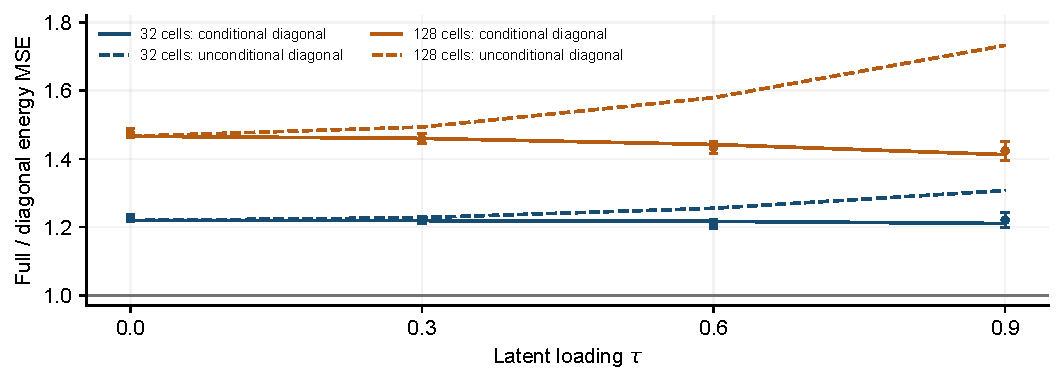
\includegraphics[width=\linewidth]{revision/experiments/latent_correlation_sweep.pdf}
\caption{Common-factor sensitivity at seven bits per source value.
Solid curves retain the full latent mean response in the diagonal comparison;
dashed curves also remove unconditional off-diagonal covariances. Markers
and nominal $95\%$ intervals use independent source vectors.}
\label{fig:latent-sensitivity}
\end{figure}
